\newcommand{\FigBentSolenoidRelativeDrift}{
\begin{figure}[t]
\centering
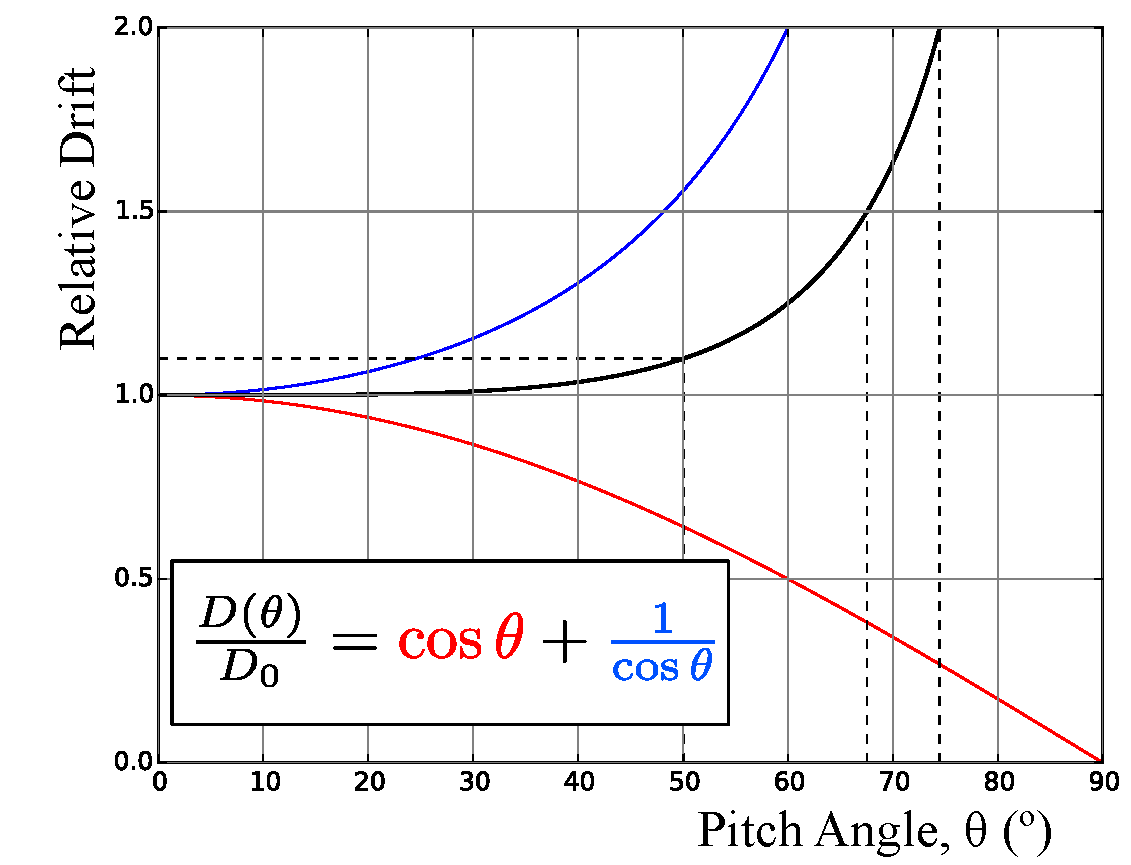
\includegraphics[width=0.6\textwidth]{figs/detector/BentSolenoids_RelativeDrift}
\caption{
Angular dependence of the magnitude of vertical drift in a bent solenoid field.
The total variation (black) remains below 10\% for pitch angles below 50\degree.
}
\figlabel{detector:bent-solenoids:angularDependence}
\end{figure}
}

\newcommand{\FigPhaseII}{
\begin{figure}[t]
\centering
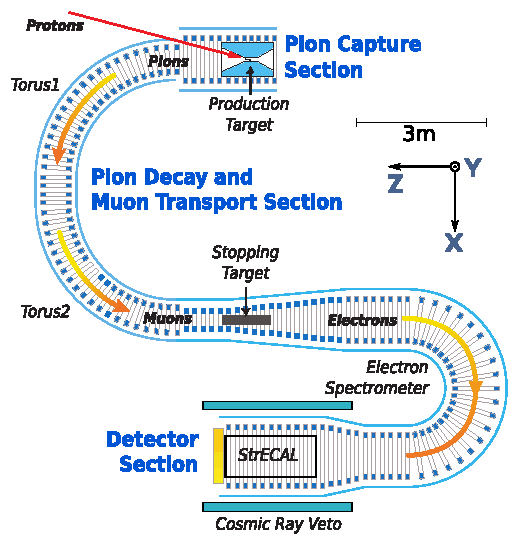
\includegraphics[width=0.9\textwidth]{figs/detector/PhaseII_schematic}
\caption{
Schematic layout of COMET \phaseII. 
The 8 GeV proton beam enters from the top-left, producing (amongst other things) pions.
Pions and muons travelling backwards with respect to the proton beam are then transported around 180 degrees of bent solenoid, during which time most of the pions decay producing an intense muon beam.
About 40\% of these muons then stop in the stopping target (centre of image).
Any electrons coming from  \mueconv are then transported through another 180 degrees of bent solenoid into the detector system.
}
\figlabel{detector:PhaseII:setup}
\end{figure}
}

\newcommand{\FigPhaseI}{
\begin{figure}[t]
\centering
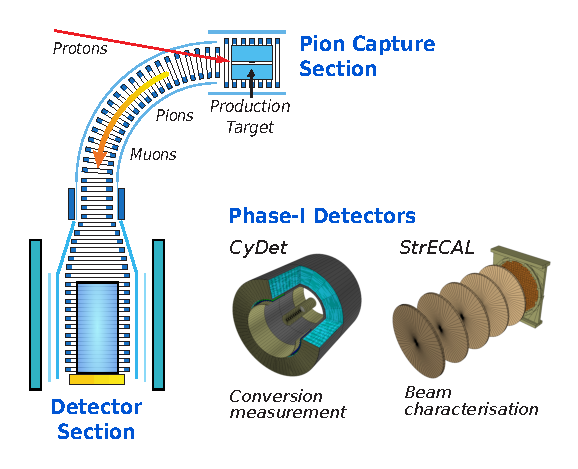
\includegraphics[height=0.4\textheight]{figs/detector/PhaseI_schematic}
\caption{
Schematic layout of COMET \phaseI. 
}
\figlabel{detector:PhaseI:setup}
\end{figure}
}

\newcommand{\TabBackgroundSummary}{
\begin{table}
\begin{tabular}{lldd}
     \hline
     \hline\\[-1.8ex]
     Type           & Background & \multicolumn{2}{c}{Predicted number of events during run} \\
                    &  & \multicolumn{1}{c}{\phaseI \cite{TDR2014}} & \multicolumn{1}{c}{\phaseII \cite{CDRphase2} } \\
     \hline\\[-1.8ex]
     Intrinsic & Muon Decay-in-Orbit                       & 0.01              & 0.15    \\
               & Radiative Muon Capture                    & 0.00056           & <0.001  \\
               & $\mu^-$ Capture w/ n Emission             & <0.001            & <0.001  \\
               & $\mu^-$ Capture w/ Charged Part. Emission & <0.001            & <0.001  \\
     Prompt    & Radiative Pion Capture                    & 0.00023           & 0.05    \\
               & Beam Electrons                            & 0.00083           & <0.1^*  \\
               & Muon Decay in Flight                      & \le0.0002         & <0.0002 \\
               & Pion Decay in Flight                      & \le0.00023        & <0.0001 \\
               & Neutron Induced                           & -                 & 0.024   \\
               & Other beam induced B.G.                   & <2.8\times10^{-6} & -       \\
     Delayed   & Delayed Radiative Pion Capture            & \sim0             & 0.002   \\
               & Anti-proton Induced                        & 0.007             & 0.007   \\
               & Other delayed B.G.                        & \sim0             & -       \\
     Cosmic    & Cosmic Ray Muons                          & -                 & 0.002   \\
               & Electrons from Cosmic Ray Muons           & <0.0001           & 0.002   \\
     \hline\\[-1.8ex]
     \multicolumn{2}{c}{Total background}                      & 0.019         & 0.34    \\
     \multicolumn{2}{c}{Signal (Assuming $B=1\times10^{-16}$)} & 0.31          & 3.8     \\
     \hline
     \hline
\end{tabular}
\caption{
	\CHECK{UPDATE \phaseI values with TDR 2016}
	Backgrounds for COMET \phaseI \cite{TDR2014} and \phaseII \cite{CDRphase2}.
	Prompt backgrounds arise by protons that occur in between bunches and are therefore suppressed by the extinction factor.
	For \phaseI, the recently measured value of $10^{-12}$ was used for the extinction factor, but for \phaseII the older expectation of $10^{-9}$ was used.
}
\tablabel{detector:backgrounds}
\end{table}
}

\newcommand{\FigMuonNuclearParams}{
\begin{figure}[bp]
\centering
\subfloat[][\figlabel{detector:mu-nucl-params:lifetimes}Lifetimes]{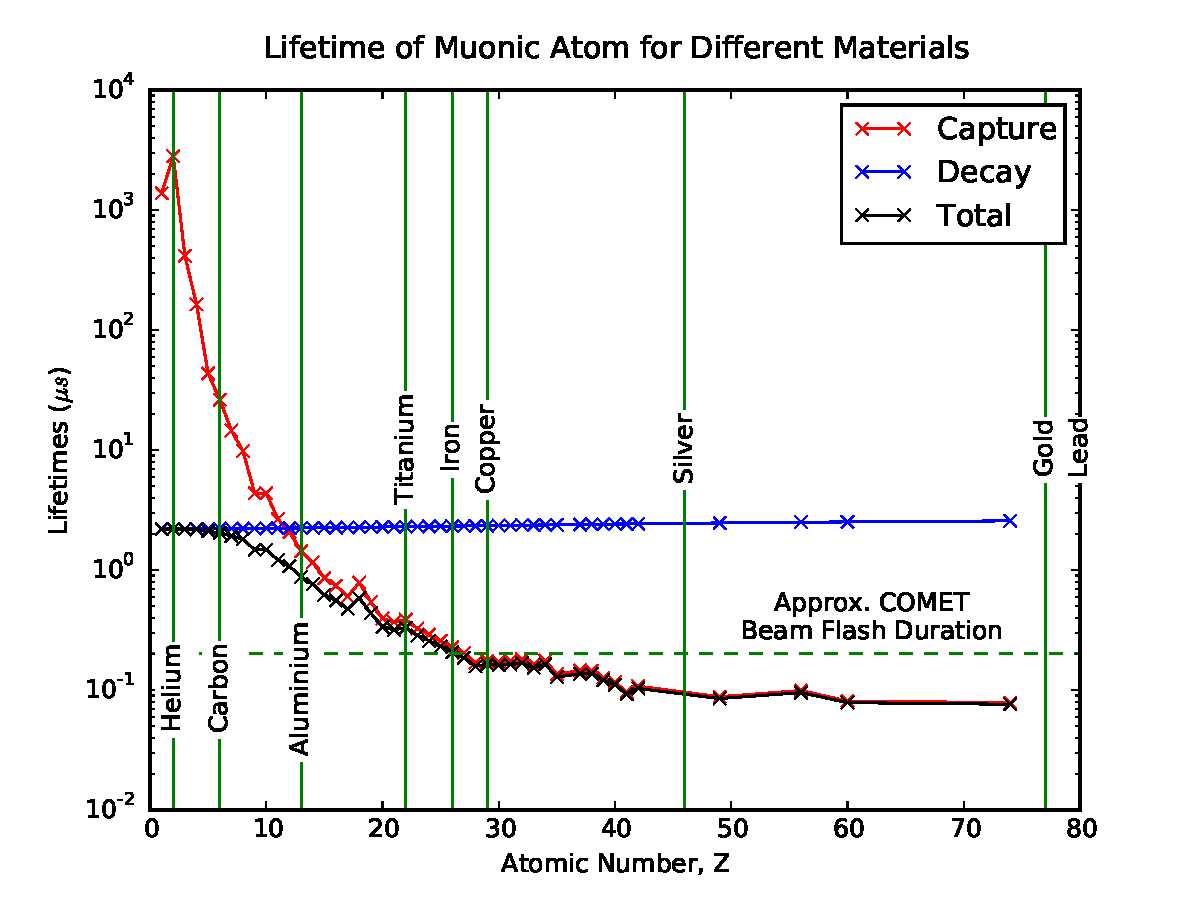
\includegraphics[width=0.9\textwidth]{figs/detector/MuNuclearParams_All_lifetimes.pdf}}\\
\subfloat[][\figlabel{detector:mu-nucl-params:end-point}End-point Shift]{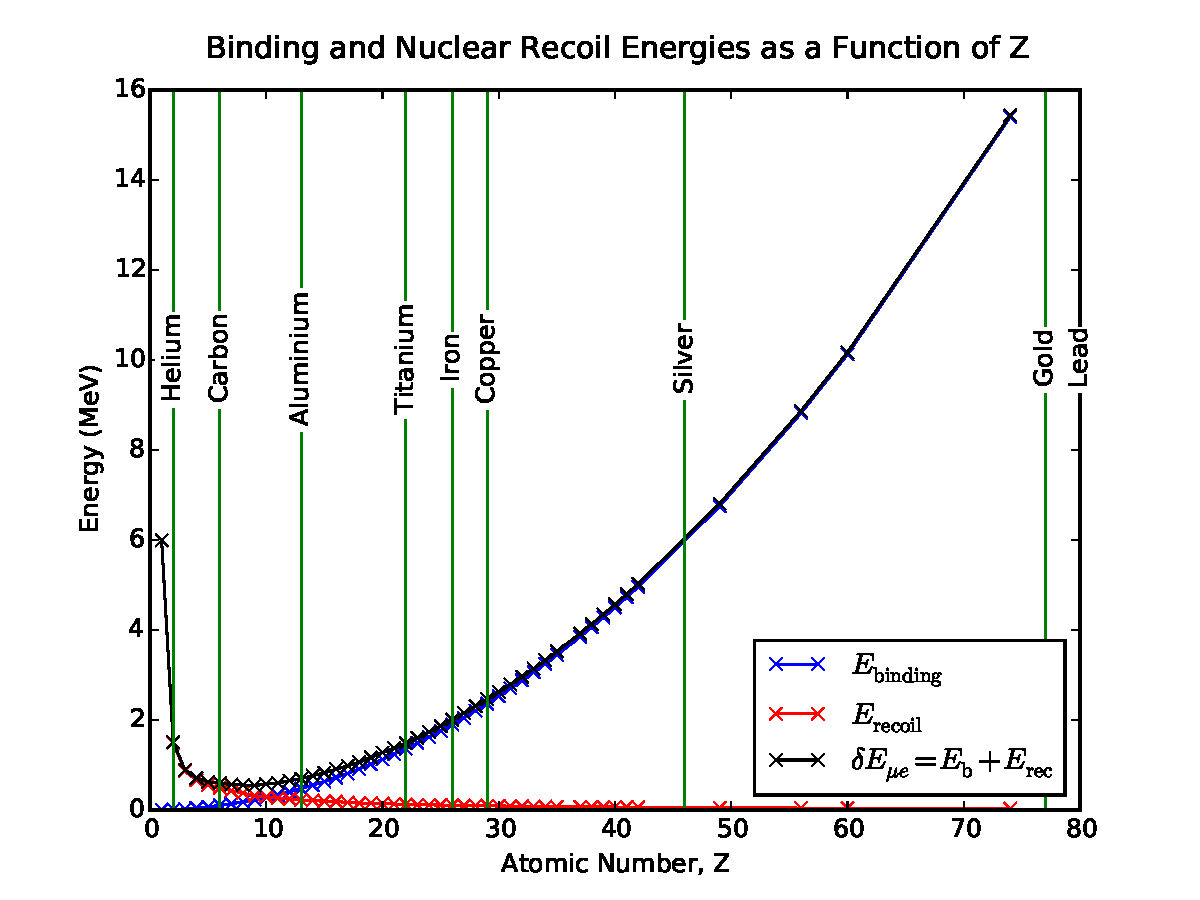
\includegraphics[width=0.49\textwidth]{figs/detector/MuNuclearParams_energies.pdf}}%\hspace{0.5cm}%
\subfloat[][\figlabel{detector:mu-nucl-params:branching-ratio}Branching Fraction]{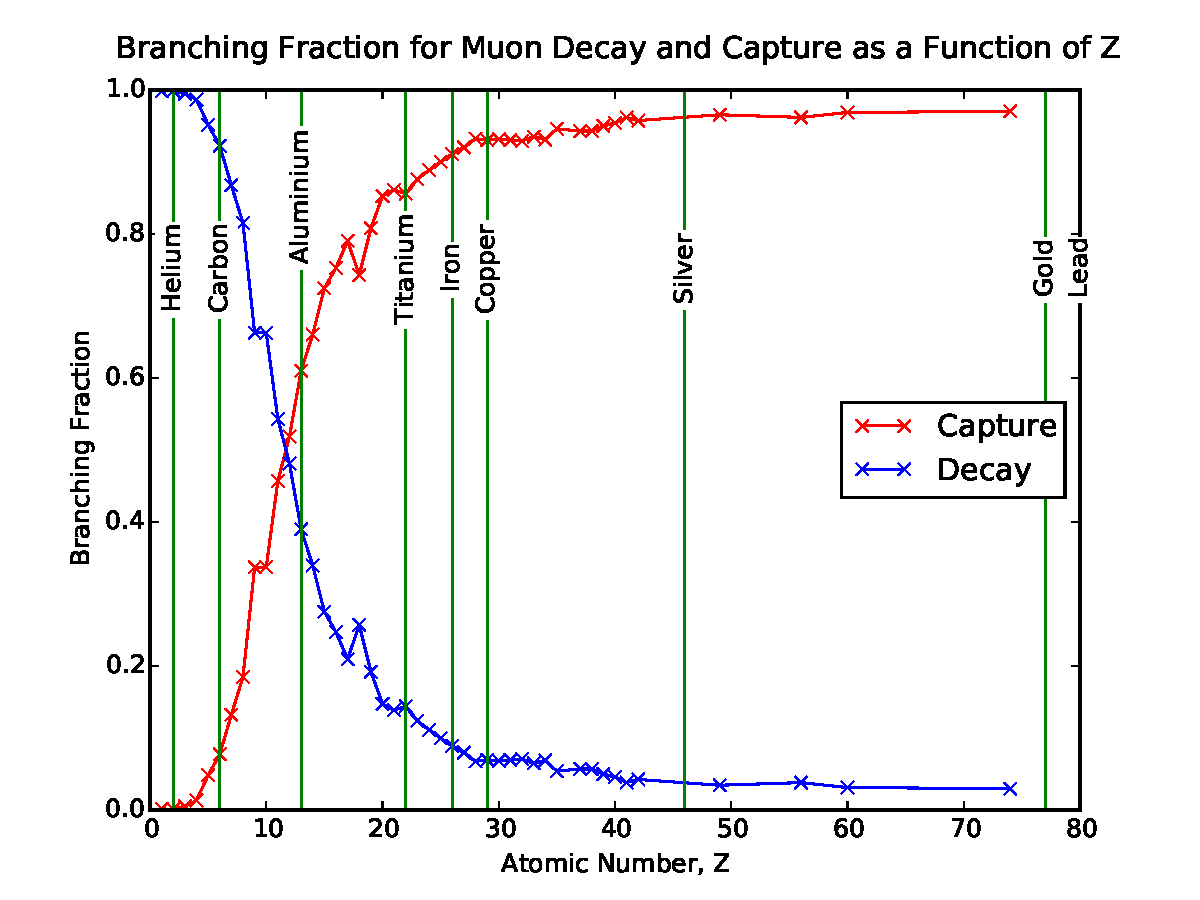
\includegraphics[width=0.49\textwidth]{figs/detector/MuNuclearParams_branching_fraction.pdf}}
\caption{\figlabel{detector:mu-nucl-params}
The effect of changing the atomic number on the branching ratio, lifetime and electron energy spectrum end-point.
For the branching ratio and lifetime plots, the partial rate for muon nuclear capture and decay-in-orbit are shown separately.
The capture and decay rates are taken from the Geant4 \cite{Geant42003} parametrisation for stopped negative muons.  
Only elements for which at least 1 isotope uses a measured value are plotted.
The values for the end-point energy level are calculated using the Bohr model for the muon ground-state binding energy.
}
\end{figure}
}


\chapter{The COMET Experiment}
%\section{Muon to Electron Conversion: Signal and Backgrounds}
% - COMET stands for COherent Muon to Electron Transitions
% - Cite the experimenter's guide by Bob Bernstein

%Introduction:
The COMET experiment will search for COherent Muon to Electron Transitions with a single-event sensitivity of around \sensePII.
This amounts to an improvement of four orders of magnitude compared to the current limit by \sindrumII~\cite{sindrum2006}, made possible by significant changes to the way the experiment operates compared to its predecessor.

Reaching such a sensitivity requires that COMET stops many muons in aluminium, whilst maintaining a high signal acceptance but
suppressing potential background sources to well below a single event during the lifetime of the experiment.
%\begin{itemize}
%\item stop many muons in aluminium,
%\item have a high signal acceptance,
%\item suppress potential background sources to well below a single event.
%\end{itemize}
This tension between simultaneously high signal sensitivity and background suppression can be translated into the more specific requirements of:
\begin{itemize}
\setlength{\itemsep}{-1ex}
\item a very high-intensity, low-energy, and high-purit muon beam,
%\item a low energy muon beam,
\item a thin stopping target and low material budget detector,
\item the use of timing information of signal process with respect to backgrounds.
\end{itemize}

The design of COMET realises these goals by employing several novel experimental techniques and, as such, it has been decided to operate in two stages, \phaseI and \phaseII.
\phaseI aims both to help understand these techniques, the muon beam, and key backgrounds rates, as well as making an intermediate measurement of \mueconv at a sensitivity of \sensePI---two orders of magnitude better than the \sindrumII experiment.
\phaseII will follow and should achieve the final objective of \sensePII. 
%Firstly however I will discuss some of the key aspects common to both \phaseI and \phaseII.
%Although \phaseI will run sooner, since it is heavily motivated by \phaseII, I shall describe \phaseII in more depth first and return \phaseI subsequently.

\section{Overview of Signal and Backgrounds}
\sectlabel{detector:background}
The \acf{ses}, defined in the previous chapter, is a statement purely of signal efficiency and does not account for background rates.
It is clear, however, that for any observation to be confidently labelled as signal or, in the event of a null-observation, in order to set the tightest possible confidence limit, the background rate must be kept comparably low.
In order to understand the design of the \COMET experiment, a simple appreciation of the key backgrounds is therefore necessary.
%To understand the design of both phases of COMET a simple appreciation of the signal and types of backgrounds that must be considered is necessary.

%Given the desired sensitivity of COMET is \sensePI  at \phaseI and \sensePII by \phaseII, background rates must be kept equally rare.

\TabBackgroundSummary%
\Tab{detector:backgrounds} summarizes the results of previous studies for background rates at \phaseI and \phaseII.
There are four groups of background source: intrinsic, prompt, delayed, and cosmic.

Intrinsic processes are those that arise from muons stopping in the target and will always be present regardless of the muon beam properties.
The muon \ac{DIO} which was described in the previous chapter is one such background.
%One Of these, the dominant background is muon \acf{DIO}, which was described in the previous chapter.
In addition, radiative nuclear capture of a muon is kinematically capable of producing 101.85~MeV photons, which can produce backgrounds if the photon is converted to a high-energy electron and then mis-reconstructed to have additional energy.

%Although the decay of a free muon cannot produce electrons with energy greater than half the muon mass, once bound to a nucleus the neutrinos can be configured to carry away almost no kinetic energy, leaving only the nucleus and electron to determine the kinematics of the end-point configuration.
%From this it can immediately be seen that the maximum energy of the electron produced from muon decay-in-orbit is the same as for \mueconv (up to the neutrino mass), and indeed
%a tail in the spectrum of electrons coming from muon \ac{DIO} extends all the way up to this point.
%However, clearly such a configuration occupies a tiny part of the phase space as can be seen from \fig{detector:DIOSpectrum} which shows the spectrum of electrons from muon \ac{DIO} in aluminium.
%It can be seen that whilst the high energy tail does reach up to about 105~MeV/c, the rate drops away very steeply above the free-muon decay end-point, falling some 18 orders of magnitude from its peak around 50~MeV/c.
%%Since the nucleus is so massive compared to the electron, it requires very little energy to have it conserve momentum with the outgoing electron.

Delayed and prompt processes come from impurities in the muon beam, be they pions, antiprotons, or high energy muons and electrons.
The key distinction between these two is the timing at which the background is detected with respect to the arrival of the proton beam.
For example, pions that reach the stopping target region are dangerous since they can produce high energy gamma rays which can pair produce to create 105~MeV electrons.
Since pion capture against a nucleus is extremely fast, the timing of pion-induced backgrounds is determined predominantly by the arrival time of pions into the target region.
In order to reach this region without decaying, the pions must be relatively high momentum of about 60~MeV/c or greater.  

As a result, backgrounds from pion capture are typically expected close to the arrival of protons at the production target.
Prompt processes such as this are suppressed by using a pulsed proton beam (discussed in more depth later) and ensuring very few protons in between pulses.
Other beam related issues include the decay of muons and pions to electrons.
An electron of 100~MeV/c can be produced by muons or pions with momentum greater than 70 or 50~MeV/c respectively, and so the flux of higher energy particles in the beam must also be reduced.

Delayed processes are those where the timing of the proton beam cannot be used to improve suppression since the characteristic time between the primary proton striking the target and the detection of the background for these processes is large compared to the time between beam pulses
Possible sources of this delay include the mirroring of particles by the magnetic field, or by some heavy particle from the production target producing pions and high-energy electrons.
At a given momentum, antiprotons travel considerably more slowly than muons or pions given their considerably larger mass, washing out any timing information from their production.

Finally cosmic backgrounds arise from high energy muons that pass through the building and enter the detector or beamline.  
Events where a muon decays to an electron which is then detected as 105~MeV are counted as backgrounds.
In particular, muons that produce high energy electrons close to the target are dangerous since cuts on the reconstructed direction and position will be less effective.

All these processes will be discussed and evaluated in more depth in the section on background estimates.

\section{General Experimental Techniques}
Suppressing background rates while maintaining a high signal efficiency leads to several novel techniques being used in the COMET experimental set-up.
These techniques are common to both \phaseI and \phaseII.

\subsection{Proton Beam Energy and Production Target}
The muon beam used in COMET is produced from the decay of a secondary pion beam created by protons striking a target.
If maximising the muon intensity were the only concern, then both the proton beam power and atomic mass of the target material would similarly be maximised since the pion production cross section
grows with these two parameters.
However, the need to suppress background rates and maintain the mechanical and operational stability of the target constrains both of these parameters.

In particular, protons striking an individual, stationary (and, in theory, unbound) nucleon with more than about 6~GeV have sufficient energy to produce antiprotons which travel relatively slowly (see \ref{sec:stop-tgt}) and can produce backgrounds.
Since the antiproton yield grows very quickly above this threshold, it has been chosen to use protons with 8~GeV kinetic energy.

As well as the beam energy, the intensity is ideally maximised to increase the number of protons on target per second.
For \phaseII running, the main ring will operate at 7~$\mu$A so that a beam power of 56~kW is achieved.  
\phaseI on the other hand will use a lower beam intensity of 0.4~$\mu$A or 3.2~kW.

Whilst a heavy metal target is preferable since it increases the number of nucleons that interact with the proton beam and therefore the pion yield,
the target must maintain its mechanical strength.
This requires the selection of a high melting point material and possibly the use of active cooling.
To simplify the situation in \phaseI, a graphite target will be used which can be passively cooled by thermal radiation.
In \phaseII however, tungsten has been selected due to it high melting-point of 3422 C, although water cooling will also likely be employed.

\FigPionSpectraVsAngle

Finally, only those pions and muons emitted in the backwards direction with respect to the proton beam are captured and transported to the muon beamline.
This is a strong way to reduce the high-energy components of the muon and pion distributions since the yields for low momentum pions in the forward and backwards directions are similar, whilst the high energy tail is greatly suppressed in the backwards direction.
At this time however, there is a dearth of experimental measurements for pion production in the backwards direction with 8~GeV protons on a graphite or tungsten target.
\Fig{detector:piYield} shows a measurement of the cross section for pion production with 10~GeV protons on tantalum (which is adjacent to tungsten on the periodic table).

\subsection{Particle Transport through Bent Solenoids}
Both \phaseI and II make use of bent solenoids to help select particles of a particular momentum.
When transported through a bent solenoid, charged particles are dispersed proportionally to their momentum and charge.
This creates a separation between the high and low-momentum components of the beam, such that collimators can selectively remove the high-momentum particles.

Charged particles moving through a straight solenoid follow a helical
trajectory, orbiting a point that moves parallel to the solenoidal axis with constant velocity fixed by the longitudinal momentum of the particle.
The frequency that the particle rotates about this point (the cyclotron frequency or frequency of gyration) is determined by the transverse momentum.
\FigBentSolenoidRelativeDrift

By comparison, if a charged particle moves through a solenoid channel that has been bent, the particle can still be considered to orbit a point, only now 
the motion of that point can be shown to drift vertically, out of the plane of bending.
This drift arises partially due to the gradient introduced to the field by bending the solenoid but also from the 
non-rectilinear coordinate system of the field lines.  
The total drift, $D$, of a particle with mass and charge $m$ and $q$ respectively  through a solenoid bent with a fixed radius of curvature, $R$, is given by:
\begin{align}
	D=&\frac{1}{qB}\left(\frac{s}{R}\right)\frac{p^2_\mathrm{L}+0.5p^2_\mathrm{T}}{p_\mathrm{L}}\eqlabel{detector:bent-solenoids:longVstrans}\\
	 =&\frac{1}{qB}\left(\frac{s}{R}\right)\frac{p}{2}\left(\cos\theta + \frac{1}{\cos\theta}\right)\eqlabel{detector:bent-solenoids:pitchAngle}
\end{align}
where $B$ is the magnetic field strength\footnote{Strictly speaking, $B$ is the field strength along the path of the centre of gyration, which is constant for a fixed transverse distance from the focus of the bent solenoid.},
$s$ is the distance travelled through the solenoid, $p$ the momentum of the particle, with $p_\mathrm{L}$ and $p_\mathrm{T}$ its longitudinal and transverse components with respect to the solenoid axis.
%(see appendix \ref{sec:appendix:bent-solenoid} for a full derivation of these equations). %\eq{detector:bent-solenoids:longVstrans} and \eq{detector:bent-solenoids:pitchAngle}).
The pitch angle, $\theta$, is a property of the helical trajectory taken by the particle and defined as:
\begin{equation}
\theta=\tan^{-1}\left(\frac{p_\mathrm{T}}{p_\mathrm{L}}\right)
\end{equation}
The angular dependence of equation \eq{detector:bent-solenoids:pitchAngle} is shown in
\fig{detector:bent-solenoids:angularDependence} where it can be seen that for
angles below 50 degrees the variation in the drift is less than 10\%, such that
the drift is determined almost completely by the momentum of particles up to
these angles.

Bent solenoids are used in \COMET for both \phaseI and II to disperse high-energy muons and pions in the muon
beam, and as a spectrometer system for electrons coming
from the stopping target in \phaseII, which will both be described in more
detail below.

Since the drift is proportional to the momentum of the particle, particles with zero momentum would remain on axis, whilst higher momentum particles, including those of interest (105~MeV electrons in the \phaseII electron spectrometer and around 40~MeV/c muons in the muon beam line), drift to the sides.  
However, an additional vertical component is introduced to the magnetic field.
If the solenoid were straight the axis of a particle's helical trajectory would follow the field line. 
A vertical component would, therefore, cause the trajectories to move upwards with the field line itself, irrespective of the particle's momentum.
The same result is true in a bent solenoid and since the drift this introduces is not proportional to momentum a vertical component can be used to select the momentum of particles which remain on axis.

Two techniques have been considered to introduce this vertical component: tilting the solenoid coils themselves, or adding additional dipole coils around the solenoids.
\COMET has chosen to pursue the latter, using a special, proprietary winding technique developed by Toshiba to introduce a vertical component by placing additional conductor around the solenoid coils.
Since the current through these dipole coils can be altered separately to the solenoid coils, this approach has the advantage that the two components can be tuned against each other.
This allows for the optimal dipole field to be found during operation running, and for the on-axis momentum and charge shifted to study backgrounds or other physics searches.
Additional collimator material can also be introduced to remove particles with undesirable momentum.

%The dynamics of a charged particle in a magnetic field is determined by the Lorentz equation:
%\begin{equation}
%\vec{F}=\frac{q}{m}\vec{p}\times\vec{B}
%\end{equation}
%where $q$, $\vec{p}$ and $m$ are the particle's charge, momentum and mass respectively, and $\vec{B}$ is the magnetic field.
%In a uniform magnetic field where all field lines are parallel, clearly the motion of the particle follows a helix whose axis is parallel to the field and
%with a helical pitch-angle given by:
%\begin{equation}
%\theta=\tan^{-1}\Big(\frac{P_\mathrm{T}}{P_\mathrm{L}}\Big)
%\end{equation}
%where $P_\mathrm{T}$ and $P_\mathrm{L}$ are respectively the transverse and longitudinal components of the momentum with respect to the magnetic field.
%Such a field can be realised to a high precision by a cylindrical solenoid coil.
%
%If instead one were to bend a solenoid coil, so that it's axis describes a circular arc, two effects are introduced:  firstly, the uniformity of the field is changed
%such that a higher magnetic field is found on the inside of the bend, and secondly the field lines also bend.
%Each of these changes causes the motion of the particle to deviate from that of a straight solenoid.
%Whilst one can think of the particle as following a helix around the field lines still, the centre of this helix can be shown to drift out of the plane of the bending.
%Firstly, the radial gradient introduced to the field causes a drift which is proportional to the transverse momentum of the particle.
%Secondly, the centrifugal pseudo-force as the particle tracks the now cylindrical field lines, creates a force that acts perpendicularly to the magnetic field.
%Since the field lines follow the solenoidal axis, this also produces a vertical drift, proportional to the longitudinal momentum, however.
%
%Taken together, the result is a vertical drift with a velocity given by:
%\begin{equation}
%\end{equation}

\subsection{Stopping Target Material and Beam Pulsing}
\label{sec:stop-tgt}
\FigMuonNuclearParams

The combination of using backwards going pions and the long, bent-solenoid transport channel is already effective at removing potential background issues.
In addition to these however, there is one further method which helps both to reduce beam-related backgrounds and improve the detector occupancy and reconstruction requirements:
the use of a pulsed proton beam with a relatively light stopping target.

Since the signal process is coherent, its cross section grows roughly as the square of the number of nucleons (or protons, depending on the model)%
\footnote{Although this growth is offset by the normalisation to the capture rate which is typically treated as incoherent so that it grows linearly with the number of nucleons.  The overall conversion rate itself is roughly proportional to the atomic number for lighter elements.}
until the muon is contained almost completely within the nucleus at which point the rate levels off.
It is therefore desirable to use a high-Z target in order to increase the probability of conversion and indeed \sindrumII used both lead and gold targets, with its most stringent limit set on a gold target~\cite{sindrum2006}.

However, as the nucleus gets larger, the lifetime of the muonic atom falls steeply due to the increase in the nuclear capture rate.
This is illustrated in \fig{detector:mu-nucl-params} where it can be seen that for elements heavier than iron ($Z>26$) the muon lifetime is less than 200~ns.
The COMET production target and beamline produces a beam flash that lasts for about 200~ns after the arrival of a proton.
This means that for targets heavier than iron timing information is not a useful parameter to distinguish particles in the beam from electrons coming from stopped muons.

Whilst these are the two dominant factors in deciding the target material, other factors like the mechanical stability, cost, isotopic purity and the stability of the daughter nuclei following muon capture on the target must also be considered.
Accordingly, titanium and aluminium are considered the two most viable target materials.  
Titanium, in which the muon lifetime is about 330~ns, would be considerably harder to measure \mueconv so at this stage the COMET experiment is focussed on using aluminium where the muon lifetime is about 864~ns~\cite{Suzuki1987}.

\FigTimingSchematic

The J-PARC accelerator has buckets separated by 550~ns, although separations of multiples of this number can, in principle, be achieved.
For COMET running the intention is to fill every other bucket so that pulses are separated by 1.17~$\mu$s.
\Fig{detector:timing-schema} shows the beam timing schematically.  
A window from about 700 to 1100~ns after the proton beam arrival is then used to look for signal events, by which time most of the beam flash should have passed whilst signal events remain probable.

Having a well-defined bunch structure is crucial for this scheme to work. 
Protons arriving in between bunches would produce (a fragment of) beam flash that could include high energy muons or pions.   
If these produce signal-like electrons that would a background source that the timing window would be unable to remove.
The extinction factor is used to quantify the probability of protons arriving out of time, and is given by:
\begin{equation}
	R_\mathrm{Extinction}=\frac{N(p~\mathrm{between~bunches})}{N(p~\mathrm{per~bunch})}.
\end{equation}
Original background predictions were made assuming $R_\mathrm{Extinction}$ was around $10^{-9}$~\cite{CDRphase2} (about 1 out-of-time proton for every 7 \phaseI bunches) although recent measurements have been able to demonstrate extinction at a level of $10^{-12}$~\cite{COMETExtinctionNote} (about 1 out-of-time proton for every 7100 \phaseI bunches).

The bunch structure is initially defined by the linac at J-PARC which accelerates protons up to 600~MeV.
The \ac{RCS} then takes these protons up to 3~GeV where up to two buckets can be stored, although for COMET only one bunch at a time will be filled.
The protons are then injected into the \ac{MR} which accelerates them up the final energy of 8~GeV and is capable of storing up to 9 buckets at once.
Using the linac chopper alone would not be sufficient to produce the desired extinction factor since stray protons tend to drift into the unfilled buckets.
Achieving the high extinction factor then is possible only by using the injection kicker from the \ac{RCS} to the \ac{MR} in a `double-kick' mode.
The kicker excitation length is set to two buckets (so that the \ac{RCS} is completely emptied into the \ac{MR}).  
The kicker is then activated again immediately after the first filled bunch has performed a complete rotation of the \ac{MR} such that protons that had diffused into the second bunch of the \ac{RCS} are now kicked away.
Thus only every second bucket in the \ac{MR} is filled and all other buckets are kept empty.

\section{\COMET \phaseI}
\FigPhaseI
% - Measurement goals
% - StrECAL detector
% - CyDet detector
\phaseI will see the construction of the \COMET hall, the production target capture solenoids, the first 90 degrees of the bent muon transport solenoid, and the detector solenoid.  
The beamline is shown schematically in \fig{detector:PhaseI:setup} where the two interchangeable detector systems can also be seen.

There are two key goals to \phaseI:
\begin{enumerate}
	\item measure \mueconv at a \acf{ses} of \sensePI, and
\item prepare for \phaseII by measuring the beam profile, particle yields and background rates, and prototype the detector technology.
\end{enumerate}
Since the dynamics of bent solenoids are complicated, it is important to study the beam as close to the production target as possible.
However, due to the high radiation environment around the production target, the detector and electronics cannot be placed too close and must be well shielded.
\phaseI will therefore measure the beam after the first 90 degrees of bent solenoid with the same detector system to be used in \phaseII, namely the \ac{StrECAL} detector---a series of Straw Tracker stations  followed by an ECAL
all sitting in the beam.  

However, since the StrECAL detector will be hit by the full force of the muon beam, it would not be feasible to conduct a \mueconv search using this detector.
As such, for \phaseI a second detector, known as the \ac{CyDet} will be used for this purpose.
The \ac{CyDet} uses a \ac{CDC} to reconstruct the trajectories of charged particles and a pair of Cherenkov and Scintillation counters (one upstream and one down) to trigger the read-out of the system.
The \ac{CyDet} escapes the issue of the beam flash that the \ac{StrECAL} would face at \phaseI since only the outer region is instrumented.
Since the detector sits in a 1~T solenoid field (and both the detector and solenoid are co-axial), particles follow helical trajectories with the radius of gyration determined by the transverse momentum of the particle.
The beam is introduced in the centre and typically remains in an envelope of 15~cm whilst the stopping target sits in the centre of the detector with a radius of 10~cm.
As such the detector itself is geometrically blind to charged particles in the beam and electrons coming from muon \ac{DIO} in the target with momentum less than 60~MeV/c which make up the majority of the \ac{DIO} spectrum.
To reconstruct the longitudinal position of the particle's trajectory an all-stereo configuration is used in the Cylindrical Drift Chamber, where each layer of wires is rotated in the opposite direction to the previous layer by an angle of 4\degree with respect to the solenoid axis.

Because the \phaseI detector sits much closer to the stopping target than at \phaseII, there is greater exposure to hadrons emitted following nuclear capture of the stopped negative muons, such as protons, deuterons, alpha particles and so on.
Despite being emitted with kinetic energies of a few tens of MeV, momenta above 60~MeV/c are readily achieved given the large mass of these particles.
For similar reasons these particles are typically very heavily ionising so, if left unchecked, could easily dominate the occupancy of the \ac{CDC}.
The \alcap experiment has shown that for muon capture on Al-27 nuclei, the emission of a proton occurs for about 3\% of every muon capture~\cite{NamThesis}.
At this level, it is believed that no specific shielding is required beyond the carbon inner wall of the \ac{CDC} needed to contain the gas mixture.

Four layers of scintillation bars will surround the outside of the detector to provide a veto for cosmic ray events.
The most dangerous event would be a high energy muon reaching the target and decaying to a 105~MeV electron which is then detected. 
Dedicated cosmic runs will be performed prior to operation with a beam in order to understand the flux of cosmic muons.

\section{\COMET \phaseII}
\FigPhaseII
Since chapter \sect{phaseII-optimisation} presents an in-depth optimisation of the design of \phaseII, I shall only give a brief introductory overview here, most of which is based on the design as laid out in the 2009 CDR~\cite{CDRphase2}.

COMET \phaseII will be the final stage of the experiment.
It will extend the muon beamline built for \phaseI by an extra 90\degree, and add two extra solenoid sections: one to hold the stopping target, and a second 180\degree bent solenoid with a large aperture of 60~cm radius.
This layout is shown in \fig{detector:PhaseII:setup}.
The bent solenoid after the stopping target is primarily there to remove the low energy \ac{DIO} electrons which otherwise could significantly increase the hit rate in the detector.
The final detector system for \phaseII will use the \ac{StrECAL} from \phaseI but probably with thinner diameter straw tubes, thinner straw material, and more tracking stations in order to improve the energy resolution.

The stopping target itself has typically been designed as thin disks of aluminium, followed by a beam blocker.  
Even including the growth of the beam envelope as it passes from the 3~T field in the bent muon transport solenoids to the 1~T field of the bent electron spectrometer solenoid, the beam blocker removes all line-of-sight between the entrance of the electron spectrometer and the muon transport solenoids so that most of the beam flash is prevented from reaching the detector.
The tapering of the field occurs almost completely across the target itself with the intention that signal electrons heading initially upstream will be magnetically mirrored back towards the detector.

As for \phaseI, an active cosmic ray veto will prevent triggering on events caused by cosmic muons.
At least the detector solenoid will be covered, but it is likely that both the spectrometer and the stopping target area are also contained in the veto.
In \phaseI, with the target surrounded by the detector, there is a degree of self-shielding against cosmic events. 
In \phaseII, however, this will not be the case since the target and detector are widely separated.

% - Proton beam energy
% - Proton beam timing
% - Production target and capture system
% - Bent Transport system
% - Stopping target
% - Detector system

\section{Schedule and Status}
\FigSchedule
The overall schedule for the COMET experiment is shown in \fig{detector:schedule}.
\phaseI is due to start data taking in \ac{JFY} 2018 so that construction and development is well underway.

\FigStatusFacility
At the time of writing, with regards to the facility, the building that will house the experiment is now finished, sitting to the side of the existing Hadron Hall at \ac{JPARC}.
Cooling and power supplies are being installed and the shielding for the concrete hatch area is being produced.
In the mean time the development of the new beamline to extract protons from the \ac{MR} and deliver them to the COMET area is being installed.
In particular, the Lambertson magnet which directs the protons towards COMET rather than the existing Hadron Hall has been built.
For the muon beamline, the \phaseI section of the bent muon transport solenoids has been built and installed and is now under commissioning studies.
Construction of the detector solenoid has also begun with the capture solenoids around the production target soon to begin.
A selection of photographs that show the construction of the facility and installation of the bent transport solenoid are show in \fig{detector:setup:facility}.

\FigStatusStrECAL
Much of the recent activity for the collaboration has been on the design and construction of the detector systems.
Beam tests to understand the performance and resolution of prototype ECAL crystals, straw tubes and the \ac{CDC} have taken place.
For the \ac{StrECAL}, production of all 2500 \phaseI straws has been completed and procurement of the \ac{LYSO} crystals for the ECAL is under way with some 200 or so crystals already purchased.
Aging tests of the straw tubes are on-going with straws being held for an extended duration under pressure and tension at KEK.
Beam-test data is being analysed to understand the position resolution for a given straw and the energy resolution of the ECAL although for the latter better than 5\% resolution for 105~MeV electrons has already been shown.
\Fig{detector:status:StrECAL} shows photographs of the prototypes and beam test set-ups of the Straw Tube Tracker and the ECAL.

\FigStatusCyDet
In the meantime the full \ac{CDC} has been strung, with some 20,000 wires---about 15,000 field wires of 125~$\mu$m thickness, and about 5,000 sense wires of 25~$\mu$m diameter---being inserted.
Every wire has had its tension checked using a vibrational resonance method, which showed some 90 wires were outside of design tolerances.  These have since been replaced.
In June 2016, the inner wall of the CDC was successfully inserted, completing the CDC construction, so that leak tests can begin shortly.  
\Fig{detector:status:CyDet} shows photographs from the stringing of the \ac{CDC}.
In parallel, cosmic ray tests have been used to study to the performance of CDC prototypes and analysis of the data is under way to deduce the X-T curve for the CDC cells.

In the less-tangible realm that is software and simulation, in April last year the offline software reached its first stable release, and has since been used to perform three large-scale Monte Carlo productions of \phaseI.
%The most recent production saw the simulation of around $10^{10}$~\ac{POT}, equivalent to about 20,000 bunches.  
Reconstruction algorithms, including track finding and fitting in the \ac{CDC} are under development and techniques to perform \ac{PID} using the \ac{StrECAL} in the \phaseI beam are also under development.
More discussion on the software and simulation can be found in the next chapter.
